\chapter{Pragmatic and semantic factors in syntactic variation}\label{sec:5}
\section{Focus type, Givenness, Argument structure}

In Chapter 4, I demonstrated that the alternation between full and elliptical strategies can be explained by the degree of activation of the background proposition. The choice of an elliptical answer over a full one appears closely linked to common ground (CG) management and the principle of linguistic economy. However, this hypothesis does not fully account for why, within the same language, multiple full strategies can coexist. For example, it does not explain the alternation between Spanish postverbal and preverbal subjects, or the variation among different cleft forms in French, such as \textit{c’est}, \textit{il y a}, or pseudo-clefts, when these structures compete to fulfil the same information-structural function. \\
Put differently, if different syntactic strategies can express narrow subject focus, what drives their selection? Can linguistic or contextual cues account for both language-internal and cross-linguistic variation?
While some authors claim that the alternation among different variants is a matter of ``true optionality” (e.g., Akmajian argues that it-clefts and pseudo-clefts “are synonymous, share the same presuppositions,  answer  the  same questions”; \cite[149]{akmajian1970deriving}), others defend the idea that the occurrence of more than one format within the same language is instead regulated by specific factors, some of which, interestingly,  overlap for both French and Spanish.\\
As mentioned in Chapter 2, in Spanish, the alternation between the SV/VS order has been generally attributed to the \textbf{type of focus} expressed: while postverbal subjects (VS) would be mostly associated with a non-contrastive reading (information), preverbal subjects (SV) have been generally reported as instances of contrastive or corrective focus (for instance \cite{zubizarreta1998prosody, costa2001postverbal, gutierrez2013structural}). \\
Similarly, focus type has been claimed to be responsible also for the alternation among different cleft types in French. \textcite{de2015status}, for instance, state that the semantic distinction between the ``exhaustive” and the ``listing” interpretation of identificational sentences is syntactically expressed via two different kinds of cleft constructions in spoken French. The exhaustive reading is encoded through the \textit{c’est}-cleft construction (\textit{C’est les enfants qui sont allés a l’ecole} `It is the children who went to school'), while the listing reading is expressed via the \textit{il y a}-cleft construction (\textit{Il y a les enfants qui sont allés a l’ecole} `There  are  the  children  that went to school'). Moreover, such a view is supported by \textcite{karssenberg2017oiseaux} in her empirical analysis of \textit{il y a} clefts with a focus-background partition.\\
Another factor that has been claimed to be relevant for the two languages is the \textbf{information status} (givenness) \parencite{firbas1966non, chafe1970meaning, prince1992zpg} of the subject itself. Givenness refers to “information the speaker believes the listener already knows and accepts as true”, and new is “information the speaker believes the listener does not yet know” \parencite[3]{clark1977}. As already mentioned in Chapter 1, subjects are generally given entities, usually known by both speaker and hearer, or in some way bridged to one of the interlocutors (e.g., \textit{A friend of mine lives in this district}). Thus, occurrences of new subjects are less frequent in spontaneous speech and, in many languages, receive a special marking. Spanish, for instance, is said to position the subject in the postverbal slot when this is brand-new, while the preverbal position is usually reserved to highly-activated subject referents \parencite{gutierrez2013structural}. Similarly, it is often claimed that spoken French disallows brand-new subjects  in sentence-initial position (also referred to as ``bad subjects” in the literature; e.g., \cite{beaver2005bad, karssenberg20186}), and resorts to special constructions to avoid uttering the new referent sentence-initially \parencite{lambrecht2010constraints}. \textit{Il y a} clefts, for instance, would be one of these strategies: by means of this particular syntactic construction, the new subject does not appear as the first element uttered, but rather after the verb \textit{avoir}, thus avoiding the sentence-initial placement.  Along the same lines, \textcite{dufter201614} argue that ``it-clefts are preferred with shorter constituents such as pro-forms,  whereas pseudo-clefts more readily accommodate longer,  in particular clausal, elements in the clefted position” \parencite[24]{dufter201614}.\\
Finally, a third relevant factor is the \textbf{argument structure} of the verb. As mentioned in Chapter 2, the different thematic roles that different types of verbs assign to their subjects (and objects) are generally said to affect not only the realization of the arguments itself (linking), but also the order in which these arguments appear within the sentence. For instance, Spanish OE-psych verbs, such as \textit{molestar} `to disturb, to annoy' display a word order where the object (whether direct or indirect) precedes the subject. This is generally attributed to the direct object being an {\fontfamily{qcr}\selectfont EXPERIENCER}, a thematic role with proto-agent properties \parencite{dowty1991thematic}. Similarly, formal syntacticians regularly claim that VS is the most natural  word  order in sentences containing an unaccusative verb, due to the fact that the subject of an unaccusative verb originates in the postverbal  position (see, for instance, \cite{burzio1986italian, rizzi1982issues, belletti1988case}). Although the naturalness with which unaccusative verbs allow inversion could be related to the position in which their subjects are projected in syntax, it has been shown that unaccusativity itself does not provide a basis for explaining  inversion in languages like Spanish or Italian, at least in the case of ``free inversion'' (e.g., \cite{leonetti2018two}). Rather, its interaction with the information-structural properties of the sentence is the determining factor. \\
\textcite{gabriel2007fokus} provides experimental evidence for the interaction between focus and argument structure in Spanish, showing that focused subjects of transitive verbs have a higher likelihood of being realized preverbally (SV) than focused subjects of unaccusatives, where speakers overwhelmingly showed a preference for the postverbal slot. However, this tendency could be reversed when the subject is part of the topical or backgrounded portion of the sentence, causing it to appear at the beginning of the utterance. Gabriel's experiments demonstrate that the subject's position is not governed purely by syntactic requirements, but rather by an interaction between pragmatics and syntax. \\
Importantly, if the link between focus and argument structure has been noted for Spanish and other languages, the same reasoning has never been applied to French. Although certain authors have noted a correlation between certain verb types and certain cleft types (e.g., \cite{apotheloz2012pseudo} on the correlation between pseudo clefts and verbs of saying), such a correlation has never been systematically investigated.\\
This chapter aims at filling this gap, by investigating the role of the three aforementioned factors in relation to subject focus and how this interaction is reflected in the syntax of both languages. On one hand, the corpus study presented here tests claims previously formulated in the literature, while on the other, it introduces an innovative element to the theory of subject focus by evaluating the influence of verb type in correlation with various cleft constructions. Additionally, it explores potential interactions among the factors discussed above. For instance, it has already been suggested that given subjects tend to appear with transitive verbs, while new subjects are generally accompanied by unaccusatives (e.g., \cite{du2003preferred}). This raises the question of whether such interactions manifest in the syntax of both languages and whether this association also influences focus-marking constructions.\\
The chapter is organized as follows: section 5.2 presents the hypothesis of the study; sections 5.3, 5.4, and 5.5 outline the materials and methodology employed in the analysis. Sections 5.6 and 5.7 report the findings from the Spanish dataset, while sections 5.8 and 5.9 focus on the French data. Finally, sections 5.10 and 5.11 discuss the results and provide a brief summary of the chapter.

\section{Formulation of the hypothesis}
As discussed in the previous section, exhibiting the same IS-function is not a sufficient criterion to account for the co-existence of more than one focus-marking strategy in the same language. Rather, it is necessary to look both within and beyond the utterance to understand what determines speakers' preferences. The results of Chapter 3 revealed that, when it comes to the mapping between IS and syntax, Spanish speakers use mostly word order alternation, while French speakers showed a preference for constructional strategies. Such findings allow the formulation of the following hypothesis:\\


\textbf{H2}: If focus type, argument structure, and givenness influence the realization of focused subjects in Spanish and French, the impact of these factors will be reflected in the distinct focusing strategies employed by each language:
\begin{itemize}
    \item In Spanish, in the alternation between \textit{in situ} and postverbal subjects (SV/VS order).
    \item In French, in the alternation among different cleft types (\textit{c’est}, \textit{il y a}, pseudo).
\end{itemize}



To test this hypothesis, a corpus study was designed using data extracted from the corpus query in Chapter 3. In this study, each factor was tested individually, followed by an analysis of their interactions with the other predictors.
\section{Material}
The corpus query reported in Chapter 3 revealed 167 occurrences of postverbal subjects and 33 \textit{in situ} subjects for the Spanish side, while 237 clefts have been found in the French data. Among the latter, 109 are \textit{c'est} clefts, 98 are \textit{il y a} clefts and only 13 are pseudo clefts. Since pseudo clefts are too scarce, they have been excluded from the statistical analysis and have been discussed separately. The sentences have been annotated for i) focus type ii) givenness of the subject referent iii) argument structure of the verb. The criteria for the annotation of the three predictors are reported in the following section.

\section{Criteria for the annotation}
\subsection{Focus type}
I adopt mainly Kiss' (\citeyear{kiss1998identificational}) notions of focus types, who distinguishes between ``identificational” (exhaustive) and ``information” (non-exhaustive) focus \parencite{kiss1998identificational}. However, to avoid confusion with the term ``information focus”, already used in Chapter 3,\footnote{Recall that, in Chapter 3, this term indicates any instances of new information filling the wh-element contained in the QUD, whether exhaustive or not, in line with \textcite{krifka2008basic}.} I employ the term \textbf{exhaustive focus} to refer to the cases in which the focused subject is selected among a set of alternatives of the same semantic type, thus filling the wh-variable contained in the (implicit or explicit) QUD, and excluding all the other possible alternatives contained in the set. The set itself may be open or closed. Thus, the exhaustive focus type also includes cases of contrastive or corrective foci \parencite{van2004incompatibility, steube2001correction,REPP20101333}, in line with Kiss' (\citeyear{kiss1998identificational}) definition. \\
Conversely, the term \textbf{not-exhaustive focus} is used for those instances of focused subjects that do not convey exhaustivity, but simply non-presupposed information. In other words, the focused subject that constitutes the answer to the (implicit or explicit) QUD does not automatically exclude the other alternatives of the set.
\\

\begin{table}
    \begin{tabularx}{0.9\textwidth} { 
   >{\raggedright\arraybackslash}X 
   >{\raggedright\arraybackslash} X  }
 \lsptoprule
 \textbf{Exhaustive focus} & \textbf{Not-exhaustive focus} \\
 \midrule
\small Performs exhaustive identification on a set of entities, and expresses exclusion of other explicitly-given alternatives, either by selection or correction. & \small Indicates the non-presuppositional nature of the information.\\
\midrule
Tag:   &  Tag: \\

\small {\fontfamily{qcr}\selectfont EXHAUSTIVE} & \small{\fontfamily{qcr}\selectfont NOT-EXHAUSTIVE} \\
\lspbottomrule
\end{tabularx}\\
    \caption{Focus types investigated}
    % \label{tab:my_label}
\end{table}


Similar to the previous corpus studies, each item has been extracted with the QUD it constitutes an answer to, which enables the distinction between different types of foci. Examples in both languages are reported below: \\

 
 

\ea \label{ex:5:73} Spanish
  \ea	 \textbf{Exhaustive Focus}\\
    \ea   \textit{Y, ¿Tampoco se sabe si han desaparecido o?}  \\
          `And, you don't know if they disappeared?'

          \ex \textit{No, yo creo que no han desaparecido las joyas}.\\
          `No, I think that the jewellery didn't disappear.'

          \exi{b.} \textit{Sólo ha desaparecido} {[\textit{el cuadro}]\textsubscript{\textsc{foc}}}\normalsize. \\
          `Only the painting disappeared.' \hfill (sgs Spanish, 22/196-198)
    \z

  \ex \label{ex:5:74} \textbf{Not-exhaustive focus}
    \ea  \textit{¿Quién gritaba?}\\
    `Who was screaming?'
    \ex {{[\textit{La chiquilla}]\textsubscript{\textsc{foc}}}}\normalsize.  \\
    `The little girl.'
    \exi{b.} \textit{También gritaba}  {[\textit{la chica}]\textsubscript{\textsc{foc}}}\normalsize.\\
    `Also the girl was screaming.' \hfill (sgs Spanish, 17/346-348)
    \z
  \z
\z


\ea \label{ex:5:75}  French\\
  \ea  \textbf{Exhaustive Focus}\\
    \ea \textit{Est-ce que c'est toi qui l'as découvert, ou?}\\
      `Is it you who founds it, or?'
      \ex \textit{Non,} \textit{c'est} {[\textit{sa femme}]\textsubscript{\textsc{foc}}} \normalsize \textit{qui l'a découvert}.\\
      `No, it is his wife who found him.' \hfill (sgs French, 11/29-30)
    \z

  \ex  \label{ex:5:76} \textbf{Not-exhaustive focus}
    \ea \textit{En fait, il y avait qui dans l'immeuble quand ça s'est passé}?\\
    `So, who was in the building when all this happened?'
    \ex \textit{Alors, en fait, il y avait}  {[\textit{la grand-mère du dessus}]\textsubscript{\textsc{foc}}} \normalsize \textit{qui était là}.  \\
    `So, there was the old lady from upstairs that was there.'
    \exi{b.} \textit{Il y a}  {[\textit{un étudiant au premier étage} ]\textsubscript{\textsc{foc}}} \normalsize \textit{\textbf{qui était là aussi}}.\\
    `There was a student on the first floor that was there too.'

    \hfill (sgs French, 9/261-263)
    \z
  \z
\z


Distinguishing an exhaustive from a not-exhaustive focus type can be a hard task, especially when dealing with spontaneous speech data. Interestingly, some clear-cut cases can be observed as in the case of examples (\ref{ex:5:73}) or (\ref{ex:5:76}), where adverbs such as `only' or `too' function as clear indicators of semantic exhaustivity or the lack of it, respectively. In other cases, exhaustivity is simply pragmatically conveyed by the context. \\
In line with \textcite{destruel2012french} and others \parencite{horn1981exhaustiveness, ,destruel2018interpretation, de2018experimental}, I assume that exhaustivity in clefts is not encoded semantically in the construction itself, but rather conveyed pragmatically through contextual cues. For instance, if speaker a asks `who lives in the apartment on the second floor?' and speaker b provides a value for the open variable (e.g., a young couple lives there), I consider that exhaustivity in this case is pragmatically conveyed, because the value provided by b is the only one that satisfies the wh-variable opened by a, and excludes all the other possible alternatives.\\
Some sentences, however, might be compatible with both readings and constitute, in principle, cases of both exhaustive and not-exhaustive focus. To avoid any confusion, such cases were annotated as {\fontfamily{qcr}\selectfont DOUBT}, and subsequently excluded from the analysis. Consider the following example: 

 \ea \label{ex:5:77}
\ea \textit{Est-ce que quelqu'un lui devait des sous?}\\
 `Did anyone owe her money?'
\ex \textit{Non, je crois pas, non.}\\    
`Non, I don't think so, no.'
\exi{a.} \textit{Alors  si c'est pas une histoire d'argent, si c'est pas histoire de  dépression et machin, si c'est pas une histoire d'amant}\textit{,} \textit{ça aurait pu être} {[\textit{la femme du locataire}]\textsubscript{\textsc{foc}}}\normalsize, \textit{enfin, qui aurait tué cette personne, parce qu'elle sortait avec son mari.}\\
`So, if it's not a matter of money, if it's not a matter of depression and stuff, if it's not an affair, it could have been the tenant's wife who, well, allegedly killed this person because she was dating her husband.' 

\hfill (sgs French, 60/284-286)        
\z \z


In (\ref{ex:5:77}), speaker a tries to give an answer to the implicit QUD `Who is the murderer?', which is the implicit QUD of the whole game task. However, the value provided in the clefted element (the tenant's wife) is accompanied by the conditional mood, an indicator that this value may or may not be the only possible alternative for the wh-variable contained in the implicit QUD. This case is somewhat different from a clear-cut exhaustive focus assertion, such as `It was the tenant's wife who killed the victim'. Moreover, there are not enough contextual cues to establish whether the tenant's wife committed the murder alone, or whether someone else was also involved (in which case it would be a non-exhaustive focus type). Given the presence of the conditional mood indicating probability rather than certainty, and the contextual nature of this assertion, this case has been annotated as {\fontfamily{qcr}\selectfont DOUBT}.

	 


\subsection{Givenness of subjects}
For the purpose of this study, I use the term givenness to indicate textual givenness, i.e., whether the referent has already been previously introduced in the dialogue or not. An exception to this criterion is the interlocutor (speaker a and speaker b) which are situationally-given referents. Although they have not always been formally introduced in the text, I consider them to be given in the situation. To determine the degree of givenness of the other referents, I distinguished two levels of annotation: 
\begin{itemize}
    \item {\fontfamily{qcr}\selectfont GIVEN}: the referent has already been previously mentioned in the text. This is independent of the referential form through which it appears (pronoun, proper name, definite NP). Examples (\ref{ex:5:78}) and (\ref{ex:5:100}) are provided for the two languages.

\ea \label{ex:5:78} Spanish
\ea 	\textit{Y ¿Nadie avisó al médico entonces?}\\
 `And nobody warned the doctor?'
\ex  {[\textit{Yo}]\textsubscript{\textsc{foc}}}\normalsize\textit{, cuando me he enterado, rápidamente he llamado al médico}.\\
`I called the doctor as soon as I realized what happened.' \hfill (sgs Spanish, 51/20-21)     
\z \z

\ea \label{ex:5:100} French
\ea \textit{Et, est-ce qu' il habite au-dessus des étudiants ou pas du tout?}\\
 `Is he the one living above the students or not at all?'
\ex \textit{Non, en fait.}\\    
`Actually, non.'
\exi{b.} \textit{Donc, c'est} {[\textit{Boussicot}]\textsubscript{\textsc{foc}}} \normalsize \textit{qui habite au-dessus des étudiants}.\\
`So, it's Boussicot who lives above the students.' \hfill (sgs French, 19/383-385)     
\z \z 

\item {\fontfamily{qcr}\selectfont NEW}: the subject referent is introduced for the first time in the dialogue. Here again, the criterion for the annotation is independent of the morphological form through which it appears. Although the most frequent way of introducing brand-new referents in the text is through an indefinite determiner, cases of brand-new referents accompanied by a definite NP may also be found. This usually happens when the referent, although being new, is somehow bridged either to one of the interlocutors or one of the other given characters of the story (e.g., the wife). For coherence with the main criterion of the annotation, such cases have also been annotated as {\fontfamily{qcr}\selectfont NEW}. Examples of brand-new referents for the two languages are provided below:

\ea \label{ex:5:79} Spanish
\ea \textit{Y, volviendo a las amistades mm del señor,} \textit{¿Eran?}\\
 `And, coming back to the acquaintances of the man, who were they?'
 \exi{a.} \textit{	¿Frecuentaban mucho por aquí estas amistades que usted dice que tenía?}\\
 `Did they use to come over here, these acquaintances that you say that he had?'
\ex  \textit{Bueno, normalmente cambiaban.}\\    
`Well, they change continuously.'
\exi{b.}  \textit{Pero en los últimos meses habían venido mucho} {[\textit{dos personas}]\textsubscript{\textsc{foc}}}\normalsize.\\
`But, lately, two people came more often.' \hfill (sgs Spanish, 2/277-280)        
\z \z

\ea \label{ex:5:80} French
\ea \textit{Il y a d'autres voisins qui sont rentrés ou sortis avant?}\\
 ‘Are there other people who entered or left the building before this moment?'
\ex \textit{Oui}.\\    
‘Yes.'
\exi{a.} \textit{Dites-moi qui, s'il-vous-plaît!}\\    
‘Tell me who, please!'
\exi{b.}  \textit{Non, posez les questions.}\\    
‘No, ask me specific questions.'
\exi{b.} \textit{Donc, en fait, il y a}  {[\textit{une femme qui habite au dessus}]\textsubscript{\textsc{foc}}} \normalsize \textit{qui est rentrée aussi}.\\
`So, actually, there is a woman who lives upstairs who came back as well.' \hfill (sgs French, 10/332-336)     
\z \z 

\item {\fontfamily{qcr}\selectfont HEAVY}: in both the French and the Spanish data, a small number of subjects are not entities but clausal subjects (or subject complements), which are traditionally considered to be non-referential. Given that the annotation of information status only applies to referential entities, these cases have been excluded from the analysis. An example can be found below:

\ea \label{ex:5:81} French
\ea \textit{Et toi, tu as une idée sur la question?}\\
 `And you, do you have an idea on this matter?'
\exi{a.}  \textit{Il y avait quelque chose qui te laissait prévoir que ce mec, il pourrait avoir des problèmes, ou?} \\    
`Was there something that made you think that this man could have problems, or?'
\ex \textit{Moi, ce qui me génait un peu chez lui c'est} {[\textit{le fait qu'il soit rosicrucien}]\textsubscript{\textsc{foc}}} \normalsize \textit{parce que ça lui apportait des fréquentations un peu louches.}\\
`As for me, what bothered me a little bit was that he was a Rosicrucian, because he had dubious acquaintances.' \hfill (sgs French, 78/255-257)   
\z \z 
\end{itemize}


It is worth noting, though, that these cases are almost exclusively found in French pseudo clefts, in line with the literature that associates this cleft type with long, heavy subjects \parencite{blanche1990franccais, roubaud1997sujet, calude2009cleft}.\\
An important consideration has to be made for the cases of ``bridging”. The concept was initially introduced by the work of \textcite{clark1977} to refer to the following expression: ``we bought some food for the picnic. The beer was warm”. To interpret the expression``the beer”, the reader has to find a referent not clearly expressed in the previous discourse, but can be inferred from what is given already. Here, although it is not explicitly said that we bought some beer for the picnic, the first assumption is that we did, and the beer mentioned in the second part of the utterance is included in the food which the speaker bought. What is involved in the interpretation of utterance such as this is not only encoding and decoding of syntactic and semantic information, but also pragmatic inferences to identify the intended referent of the definite noun phrase in the second sentence. \\
Thus, bridged referents are typically regarded as a subset of given entities. However, in my analysis, I do not categorize bridging cases as such due to the specific context of the dialogues. Given that the murder scene takes place in a particular building and the interviewer is the building's doorman, many — if not all — of the referents mentioned in the interviews can be seen as bridged in one way or another. For example, tenants, their relatives, and friends are inherently connected to the building and thus serve as bridged referents.\\
To avoid this underspecification, I adopt a textual rather than a pragmatic notion of +/- givenness. This means that referents are annotated as given if they have been previously mentioned in the text (the interview) and as new if they appear for the first time, regardless of whether their referring expression is phrased as ``his mother, his friend, the neighbour from above, etc.”.
 

\subsection{Argument structure}
Historically, the notion of argument structure is based on the recognition that there are no consistent semantic correlates to grammatical relations (in particular, subjects and objects) \parencite{waltereit2017argument}.
The semantic contribution made by the subject can vary according to the argument structure of the verb it accompanies. The literature \parencite{hale2002prolegomenon, levin2005argument} recognizes three basic types of verbs: transitives, unergatives and unaccusatives. Transitive verbs are those that take two arguments, a subject and a direct object (DO). Typically, the subject of transitive verbs has agentive properties. It is an {\fontfamily{qcr}\selectfont AGENT} because it functions as the initiator or causer of the action described by the verb. The direct object, on the other hand, has patient properties. It is the {\fontfamily{qcr}\selectfont THEME} or {\fontfamily{qcr}\selectfont CAUSEE} that is affected by the main action described by the verb (see \cite{dowty1991thematic} for further discussion on the properties of the {\fontfamily{qcr}\selectfont AGENT} and {\fontfamily{qcr}\selectfont PATIENT} thematic-roles). \\
The second type of verb is the intransitive verb, which occurs only with a single argument, the subject. Intransitives can be further differentiated between two kinds: unergative and unaccusative \parencite{perlmutter1978impersonal}. Whereas unaccusatives select a subject with theme properties, unergatives take agentive subjects.
Thus, while in sentences containing a prototypical transitive verb, the subject is generally considered an {\fontfamily{qcr}\selectfont AGENT}, unaccusative verbs do not assign any agentive properties to their only argument (the subject), giving it instead the theta-role of {\fontfamily{qcr}\selectfont THEME}. Similarly, in subject-experiencer psychological verbs (e.g., \textit{amar} `to love' in Spanish), the subject is an {\fontfamily{qcr}\selectfont EXPERIENCER}, while in OE-psychological verbs (e.g.,  \textit{preocupar} `to worry'), the subject is generally a {\fontfamily{qcr}\selectfont STIMULUS} or, in some analyses, a {\fontfamily{qcr}\selectfont THEME} (see, for instance, \cite{gutierrez2013structural}). \\
The annotation of argument structure conducted here does not follow strictly the theta-role criterion, but simply the number and type of arguments that each verb selects. For instance, verbs like \textit{matar a alguien} `to kill somebody' and \textit{conocer a alguien} `to get to know somebody' both select a subject and a direct object. From the theta-role perspective, however, it is possible to make a distinction between the agentivity cline of the subject in \textit{matar} `to kill' and the subject in \textit{conocer} `to get to know'. \\
Based on the classification made in \textcite{dowty1991thematic}, the difference would lie in the fact that, in the former case, subject and object display a clear-cut agent-patient asymmetry, while in the latter case, this asymmetry is somewhat blurred, because the object contains some proto-agent properties as well.
For the purpose of my analysis, these fine-grained distinctions have not been taken into account. Rather, I have conducted a classification in ``macro-categories”, based on the fact that both verbs select a subject and a direct object, albeit with slightly different degrees of agentivity. Thus, verbs like \textit{conocer} `to know someone' and \textit{matar} `to kill' have been both annotated as transitives, disregarding the micro-differences in their agentivity level. Within the sentences investigated, 5 different verb types have been identified:
\begin{itemize}
    \item {\fontfamily{qcr}\selectfont TRANSITIVE VERBS}: two-placed verbs selecting a subject and a direct object, where the subject is generally the {\fontfamily{qcr}\selectfont AGENT} and the DO is generally the {\fontfamily{qcr}\selectfont PATIENT} (e.g., SP: \textit{encontrar} `to find'; \textit{conocer} `to get to know'; \textit{llamar} `to call'; \textit{avisar} `to warn', etc.; FR: \textit{tuer} `to kill'; \textit{retrouver} `to find'; \textit{découvrir} `to find out'; \textit{prévenir} `to warn'; \textit{ouvrir} `to open'; \textit{appeler} `to call', etc.).
    \item {\fontfamily{qcr}\selectfont UNACCUSATIVE VERBS}: verbs selecting a single argument, the subject, who does not exhibit any agentive properties. It is generally considered to be a {\fontfamily{qcr}\selectfont THEME} (e.g., SP: \textit{llegar} `to arrive'; \textit{venir} `to come', \textit{vivir} `to live', \textit{entrar} `to come in', etc. FR: \textit{venir} `to come'; \textit{aller} `to go'; \textit{habiter} `to live'; \textit{mourir} `to die'; \textit{arriver} `to arrive', etc.).
    \item {\fontfamily{qcr}\selectfont UNERGATIVE VERBS}: based on the classification made by \textcite{mendikoetxea1999construcciones} for Spanish and \textcite{legendre1989unaccusativity} for French, unergatives are verbs that select only one argument, the subject, which, unlike unaccusatives verbs, exhibits proto-agent properties (eg. SP: \textit{gritar} `to yell'; \textit{quejarse} `to complain'; \textit{trabajar} `to work', etc. FR: \textit{agir} `to act'; \textit{se plaindre} `to complain').
    \item {\fontfamily{qcr}\selectfont OE-PSYCH VERBS}: like transitive (or also ditransitive) verbs, object-experiencer psych two-placed verbs are verbs that select a subject and a direct or an indirect object. The peculiarity of these verbs is that the (direct or indirect) object has the thematic role of {\fontfamily{qcr}\selectfont EXPERIENCER}, while the subject is the {\fontfamily{qcr}\selectfont STIMULUS} or, for some authors (cf. \cite{gutierrez2013structural}), the {\fontfamily{qcr}\selectfont THEME} (e.g., SP: \textit{gustar} `to like'; \textit{molestar} `to bother'; FR: \textit{frapper} `to struck'; \textit{étonner} `to surprise'; \textit{marquer} `to impress').
    \item {\fontfamily{qcr}\selectfont COPULAR VERBS}: copular verbs or simply copulas and attributes (e.g., SP: \textit{ser unas ocho personas} `to be more or less eight people'; FR: \textit{être un ami} `to be a friend', \textit{devenir} `to become').
\end{itemize}


Some problematic cases are due to the polysemy of the verb \textit{être} `to be' in French. Although these types of verbs are generally used as copulas and accompanied by attributes, some speakers employ them in place of other verbs, such as \textit{habiter} `to live' (e.g., 
\textit{Il y a une femme qui est au troisième étage} `there is a woman living on the third floor').\\
In this case, it is possible to observe a mismatch between the lexical semantics of the verb and the pragmatic use that speakers make of it. In other words, the verb \textit{être} does not convey the original meaning of `to be' but `to live'. Given the lack of attributes, from an argument structure point of view, these cases behave more as unaccusative verbs than as copulas. Thus, they have been annotated as {\fontfamily{qcr}\selectfont UNACCUSATIVES}.


\section{Methodology}

In the first part of the analysis, I conducted descriptive statistics in order to investigate the simple effect of each independent variable (focus type, subject-givenness and argument structure) on the dependent variable of each language (occurrences of SV/VS for Spanish, and of \textit{c'est}/\textit{il y a} clefts for French).
In experimental settings, each participant is generally required to produce one single observation for every stimulus. This guarantees that the assumption of statistical independence is not violated. Independence means that the value of one observation does not influence or affect the value of other observations. Independent data items are thus not connected with one another in any way. Conversely,  non-independent observations introduce bias and can make statistical tests give false positives. Since my analysis builds on interviews where one participant can produce more than one single occurrence of subject focus, the independence assumption cannot be respected. This implies that, since the same speaker can utter more than one critical item, data produced by the same speaker are expected to show similarities.\\
To provide a solution for this problem and demonstrate the significance of the results, I conducted inferential statistics as well. Statistical inference uses data from a sample of individuals to reach conclusions about the whole population. Inferential statistics were carried out by running a generalized linear mixed-effects model with the answer type as a dependent variable. As random intercepts, I included the interview number, which corresponds to each speaker. Including the interview number allowed me to check whether there are any possible clusters in the data, and hence if the results are statistically significant.\\
In the second part of the analysis, I investigated different levels of interactions. As a first step, I analysed the interaction between argument structure and givenness of the subject, to check whether the interaction of the two factors increases or decreases the probability to choose one syntactic construction or the other. It is generally acknowledged that given subjects tend to appear with transitive verbs, while new subjects are generally accompanied by unaccusatives (e.g., the ``Preferred Argument Structure” (PAS), \cite{du2003preferred}). Since this hypothesis has already been formulated in the literature, analysing the interaction between the verb type and the information status of the subject referent is mostly a confirmatory study. Subsequently, I investigated the interaction among my three predictors. Unlike the previous interaction, I do not have a specific hypothesis for this part of the study. Therefore, the three-way interaction has an exploratory, rather than confirmatory, nature.
All significance tests were analysed using the lme4 package \parencite{bates2014fitting} in R \parencite{rcoreteam19}. The model converged in all the cases analysed except for one (in the Spanish data set, the main effect of focus type on cleft type). For this case, I ran logistic regression instead, and did not include the random intercept.\footnote{A closer look at the counts of each interview revealed that the model did not converge because of the elevated number of interviews containing only 1 observation per interview.} In the following sections, I report the results of the main effects and the interaction effects for each language.


\section{Spanish subject position: results}
In this section, the results of the influence of each factor on Spanish subject position are reported and discussed. As already announced in Chapter 3, the tag {\fontfamily{qcr}\selectfont IN SITU} indicates the case in which the subject precedes the verb, while sentences where the subject follows the verb are tagged as {\fontfamily{qcr}\selectfont POSTVERBAL}. The analysis has been carried out with 200 items, among which are 33 \textit{in situ} subjects and 167 postverbal subjects. Since the two subject positions have a different distribution in the corpus, with \textit{in situ} being scarce, statistical tests have been conducted in order to check the significance of the findings.

\subsection{Focus type and subject position}
Table 9 shows the influence of focus type on subject position. It is possible to observe that among the 33 \textit{in situ} subjects, 82\% (n=27) encode exhaustivity, while only 18\% (n=6) are not exhaustive. Similarly, in the case of the 167 postverbal subjects, 72\% (n=119) express exhaustive foci and only 28\% (n=46) are of the not-exhaustive type. Thus, with both preverbal and postverbal subjects, there is a clear tendency to express exhaustivity rather than the lack of it. Of the 200 items, 3 subject items have been annotated as {\fontfamily{qcr}\selectfont DOUBT} due to the impossibility to establish the type of focus they convey, and have excluded from the analysis.

\begin{table}[ht]
\centering
\begin{tabular}{rrr}
  \lsptoprule
 & in situ & postverbal \\ 
  \midrule
exhaustive &  27 & 118 \\ 
  not-exhaustive &   6 &  46 \\ 
   \lspbottomrule
\end{tabular}
     \caption{Spanish subject position by focus type}
\end{table}


The results of the mixed-effects model show that the effect of focus type on the variable answer type is not statistically significant (estimate = 0.59, SE = 0.58, p-value $>$ 0.05). 
Exhaustivity is generally conveyed through contextual cues, even though it is possible to find cases with focus particles such as \textit{sólo} or \textit{solamente} `only', which help in the interpretation of the sentence. Similarly, not-exhaustive foci are either pragmatically inferrable from the context or semantically conveyed through additive particles, such as \textit{también} `too'. A closer look at the data reveals that, among the 27 exhaustive preverbal subjects, 17 express new, exhaustive information and 10 contrast. As for postverbal subjects, contrast is encoded in only 12 out of 119 exhaustive focus items, which indicates that, in comparison, contrast seems to be more frequently expressed by \textit{in situ} subjects than by postverbal ones.\\
Apart from contrast, focus type, or more precisely exhaustivity, does not seem to be a decisive factor in explaining speakers' choice between preverbal or postverbal subjects in subject focus realization. Thus, according to this data, there is no observable clear-cut correlation between focus type and answer type in the Spanish data set. 

\subsection{Givenness and subject position}

In Table 10, the number of answer types by givenness of the subject referent are reported. Of the 200 items, 1 postverbal subject was tagged as {\fontfamily{qcr}\selectfont HEAVY}, and hence excluded from the counts. Among the 33 \textit{in situ} subjects, 70\% (n= 23) are previously-mentioned subjects and 30\% (n=10) are brand-new entities, whereas among the 166 postverbal items, 37\% (n=62) are given and 63\% (n=103)  are new.\\
Confidence intervals indicate that the percentage differences between \textit{in situ} and postverbal items in both the  {\fontfamily{qcr}\selectfont GIVEN} and the {\fontfamily{qcr}\selectfont NEW} condition are significant.  Additionally, the results of the mixed-effects model show that the effect of information status on answer type is statistically significant (estimate = 1.80, SE = 0.51, p-value $<$ 0.001).

\begin{table}[h]
\centering
\begin{tabular}{rrr}
  \lsptoprule
 & given & new \\ 
  \midrule
in situ &  \textbf{\cassarastrong{23}} &  10 \\
  postverbal &  61 & \textbf{\cassarastrong{103}} \\
   \lspbottomrule
\end{tabular}
\caption{Subject position by givenness}
\end{table}



Unlike the case of focus type, here it is possible to see a clear correlation between the information status of the referent and the type of answer chosen by speakers. The two answer types seem to be the mirror image of each other in this respect, showing opposite tendencies: \textit{in situ} subjects co-occur preferentially with given entities while postverbal subjects do so with new ones. 
The correlation between givenness and subject position is noticeable when the subject is new, with 103 out of 166 cases illustrating this tendency. This is not surprising, since previous studies have already identified a tendency for new subjects to appear in non-canonical positions, while highly-activated referents generally appear preverbally (see Chapter 2). \\
A closer look at the data reveals that newness can be conveyed under different forms: while the most common referring expression is an indefinite NP (e.g., \textit{un señor importante} `an important man'), cases where a new subject is expressed by a definite NP can also be found:

\ea \label{ex:5:82}
\ea \textit{¿Quién ha fallecido?}\\
 ‘Who died?'
\ex  \textit{Ha fallecido} {[\textit{la chica del segundo}]\textsubscript{\textsc{foc}}}\normalsize.\\
‘The girl from the second floor died.' \hfill (sgs Spanish, 08/30-31)     
\z \z


In (\ref{ex:5:82}), the referent contained in the answer \textit{la chica del segundo} `the girl from the second floor' is a referent that has not previously mentioned in the discourse. Recall that the interviewer is also the doorman of the building in which the (alleged) murder has been committed. In the dialogue in (\ref{ex:5:82}), speaker a, who has been informed of a murder, asks who has died. Speaker b introduces the referent for the first time by using a definite NP. It could be argued that this choice is motivated by the fact that \textit{la chica del segundo} is somehow contextually-bridged by the situation (i.e., the building). Looking further up in the context, in any case, it is clear that the referent has not been introduced before, and is therefore new.
Among the given entities, on the other hand, it is possible to find a majority of pronouns and definite NPs. The fact that ``light” linguistic elements, such as pronouns, are mostly associated with the preverbal position is also not surprising (see section 5.1 of the present Chapter). Thus, so far the results seem to reflect tendencies already discussed in the literature with respect to the interplay between syntax and information status.


\subsection{Argument structure and subject position}
Table 11 reports the proportions of answer choice by verb type (or argument structure). Among the 200 items, the graph shows a majority of unaccusative verbs (n=123), followed by transitive verbs (n=49), some OE-psychological verbs (n=14), a few unergative verbs (n=11) and only 3 copular verbs. In this case, the absolute frequencies are presented, rather than the relative ones. 
As for the distribution between preverbal and postverbal subjects, the strongest observable association is between unaccusative verbs and postverbal subjects (69\%, n=110), while some cases of postverbal with transitives (18\%, n=31), OE-psychs (7\%, n=14), unergatives (4\%, n=9) and copular (2\%, n=3) can also be found. \textit{In situs}, on the other hand, appear to be transitive (55\%, n=18), unaccusative (40\%, n=13) and unergative (5\%, n=2). Statistical tests showed that the effect of verb type on the position of the subject is again significant (estimate = 1.90, SE = 0.54, p-value $<$ 0.001).\\

\begin{table}
\fittable{
\begin{tabular}{rrrrrr}
  \lsptoprule
 & copular & OE\_psych & transitive & unaccusative & unergative \\ 
  \midrule
in situ (n=33) &   0 &   0 &  \textbf{\cassarastrong{18}} &  13 &   2 \\
  postverbal (n=167) &   3 &  14 &  31 & \textbf{\cassarastrong{110}} &   9 \\
   \lspbottomrule
\end{tabular}
}
\caption{Spanish subject position by argument structure}
\end{table}



Although a slight preference can be observed for preverbal subjects in the case of transitive verbs, this tendency is not as clear-cut as in the case of unaccusatives and postverbal subjects. Thus, preverbal foci seem to combine with both monoargumental and transitive verbs, while no case has been found in correlation to OE-psychological verbs or copular ones. 
The fact that unaccusatives combine with postverbal subjects is again not surprising, as this tendency has already been observed for several Romance languages (see section 5.1). \\
It is interesting to note, however, that this is more a tendency rather than a deterministic correlation, as some cases of preverbal subjects can also be found with unaccusatives. A closer look at the 13 cases of preverbal subjects with unaccusative verbs reveals that there is an almost equal distribution between contrastive (n=6) and non-contrastive foci (n=7), showing that contrast alone cannot be responsible for this correlation.

\section{Multifactorial analysis: interaction of predictors for the Spanish dataset}

This section presents the results of the multifactorial analysis conducted on the Spanish and French datasets. Section 5.7.1 examines the interaction between verb type and different degrees of givenness, while Section 5.7.2 extends the analysis by including exhaustivity as a factor. Although the limited size of the data does not permit strong generalizations, the statistical results suggest a correlation between postverbal position and the combination of unaccusativity with subject newness, in line with tendencies already noted in the literature (e.g., PAS, \cite{du2003preferred}). 

\subsection{Two-factor interaction: verb type and givenness}
This section explores the interaction between verb type and the givenness of the subject referent, aiming to confirm or reject the hypothesis, widely discussed in the literature, that given subjects tend to occur with transitive verbs, whereas new subjects are generally associated with unaccusatives (PAS, \cite{du2003preferred}). The goal is to determine whether these tendencies are reflected in the syntactic structure of the language when subject focus is expressed.
As previously noted, unergative verbs, OE-psychs, and copular verbs were too infrequent to be included in the statistical analysis and were therefore excluded. Consequently, the interaction between verb type and givenness generates four possible conditions: {\fontfamily{qcr}\selectfont GIVEN-TRANSITIVE}', {\fontfamily{qcr}\selectfont GIVEN-UNACCUSATIVE}', {\fontfamily{qcr}\selectfont NEW-TRANSITIVE}', and {\fontfamily{qcr}\selectfont NEW-UNACCUSATIVE}'. \\
To assess whether the interaction effects are statistically significant, I performed a logistic mixed-effects model analysis, with the choice of answer as the dependent variable, including the interview number as a random effect.\\
Figure 5 shows the results for the Spanish data set. The data reveals that among 39 given-transitives, 36\% (n=14) are \textit{in situ} subjects, while 64\% (n=25) are postverbal; the given-unaccusative interaction resulted in 30 items, 27\% (n=8) of which are \textit{in situ} subjects and 73\% (n=22) postverbal ones. In the new-transitive combination, it is possible to find 10 items, 40\% (n=4) of which are \textit{in situ} and 60\% (n=6) of which are postverbal. Finally, the combination of new and unaccusatives was found to be the most frequent one, with a total of 91 items, 6\% (n=5) of which are \textit{in situ} and 94\% (n=86) are postverbal. A mixed-effects model showed that the interaction effect of the two variables on answer type is statistically significant for this Spanish data set (estimate = 2.40, SE = 1.15, p-value $<$  0.05).

\begin{figure}[ht]
\centering
    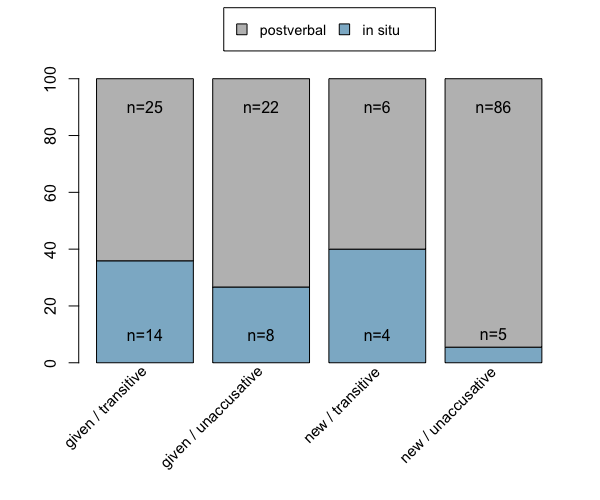
\includegraphics[width=0.7\textwidth]{Images/ES_interaction.png}
    \caption{Interaction of givenness and argument structure}
    \label{fig:5:Plot1}
\end{figure} 



By comparing the proportions of \textit{in situ} subjects, it is possible to observe a rather homogeneous distribution in the given-unaccusative, new-unaccusative and new-transitive conditions, while almost the half of \textit{in situ} (14 out of 31\footnote{Recall that 31 represents the totality of \textit{in situ} subjects without the items containing unergatives.}) contain transitive verbs with given subjects.\\
The comparison of the distributions of postverbal subjects in the different conditions, on the other hand, results in a much clearer tendency: if no significant difference can be observed between the shares of postverbal subjects in the given-transitives (n=25) and given-unaccusative (n=22) conditions, only 6 out of 139 postverbal subjects\footnote{The totality of postverbal subjects containing transitive and unaccusative verbs was originally 141 (see Table 11) However, only 139 have been used to conduct the analysis reported in Figure 5, since 2 items have been annotated as doubt.} were found in the new-transitive condition, while the vast majority (n=86) belongs to the new-unaccusative interaction.
Thus, if the subject is given, its interaction with either a transitive or an accusative verb does not lead to significant differences in the choice of the answer type. Conversely, if the subject is new, the effect of verb type is clearly visible, and the presence of new entities accompanied by unaccusative verbs strongly enhances the likelihood that speakers will choose a postverbal subject.

\subsection{Three-factor interaction}
This section explores the interactions among all three predictors. Unlike the two-factor interaction, no specific hypothesis has been formulated here. Rather, this part aims at simply exploring how different focus types interact with the other two factors. The analysis has been conducted in R \parencite{rcoreteam19}. However, due to the scarcity of the data, it was not possible to carry out inferential statistics on this data set.\footnote{Because of the few items that would result from each interaction, a mixed-effects model would not have converged. Thus, no random effect has been added to this analysis, and the statistics have been carried out descriptively.}\\

\begin{table}
\begin{tabular}[t]{lllrr}
\lsptoprule
Focus type & Verb type & Information status & In situ & Postverbal\\
\midrule
exhaustive & transitive & given & 14 & 25\\
& & new &  3 & 3\\
& unaccusative & given & 7 & 19\\
& & new & 2 & 60\\
not-exhaustive & transitive & given & 0 & 0\\
 & & new & 1 & 3\\
& unaccusative & given & 1 & 3\\
& & new & 3 & 26\\
\midrule
\textbf{Total} & & & 31 & 139\\
\lspbottomrule
\end{tabular}
\caption{
% \label{tab:}
Interaction of focus type, verb type and information status.}
\end{table}


Table 12 presents the results for the interaction of exhaustive vs. non-exhaustive focus, verb types, and the subject's information status, with raw counts indicated. As shown, many combinations yielded very few items, and some produced none at all. For example, there are no occurrences of non-exhaustive foci with transitive verbs and given subjects.
The most frequent pattern is the association between unaccusative verbs and new subjects, a finding consistent with previous analyses. Additionally, in both exhaustive and non-exhaustive conditions, this combination often results in postverbal subjects. Thus, unaccusatives paired with new subjects tend to appear as postverbal, regardless of the focus type. The interaction with exhaustivity seems irrelevant in this regard.
For the remaining conditions, some combinations produced as few as three items, with others having only one or no observations. As a result, comparisons between these conditions and the focus type interaction are not feasible.
In summary, the analysis does not permit significant conclusions due to the limited data.\\
The next section presents the results for the French dataset. As with Spanish, I first examine the individual effects of each predictor before addressing their interactions.


\section{French cleft types: results}
In this section, I present and discuss the findings from the French dataset, following the same structure as the Spanish results. I first examine the correlation between answer type and focus type, followed by information status, and finally, argument structure. As mentioned earlier, the corpus query in Chapter 3 revealed 220 clefts: 109 are c’est clefts (tagged {\fontfamily{qcr}\selectfont C'EST}), 98 are \textit{il y a} clefts (tagged {\fontfamily{qcr}\selectfont IL Y A}), and only 13 are pseudo clefts. Due to their scarcity, pseudo clefts are not represented in the graphs but are discussed separately based on their properties.


\subsection{Focus type and cleft type}
Among the 109 \textit{c'est} clefts, 1 was annotated as {\fontfamily{qcr}\selectfont DOUBT} and thus excluded from the analysis. As shown in Table 13, of the remaining 108 \textit{c'est} clefts, 99\% (n=107) express exhaustive focus, while only 1\% (n=1) belongs to the non-exhaustive focus type. Regarding the \textit{il y a} format, out of 98 \textit{il y a} clefts, 34\% (n=33) are exhaustive, while almost twice as many (66\%, n=65) are non-exhaustive foci. Logistic regression showed a significant main effect of focus type on cleft type (estimate = 5.43, std. error = 1.03, p $<$ 0.001).\footnote{I attempted a mixed-effects model, but it did not converge in this case. Therefore, I simplified the analysis by eliminating the random intercept and using a logistic regression instead. As a result, the significance of the effect should be interpreted with caution.}

\begin{table}[ht]
\centering
\begin{tabular}{rrr}
  \lsptoprule
 & \textit{c'est} & \textit{il y a} \\ 
  \midrule
exhaustive & \textbf{\cassarastrong{107}} &  33 \\
  not-exhaustive &   6 & \textbf{\cassarastrong{65}} \\
   \lspbottomrule
\end{tabular}
\caption{Cleft type by focus type}
\end{table}


The graph shows a clear-cut correlation between focus type and cleft type, where \textit{c'est} clefts encode almost exclusively an exhaustive focus type, while the majority of \textit{il y a} clefts express not-exhaustive focus, even though some cases of exhaustivity can also be found. In this respect, there seems to be a ``division of labour” between \textit{c'est} and \textit{il y a} clefts in encoding focus type. Among the 107 \textit{c'est} clefts associated with an exhaustive interpretation, 43 express contrast, while the majority encode new exhaustive information. The number of contrastive foci associated with \textit{il y a} clefts, on the other hand, was extremely low (2 out of 33), suggesting that there might be a tendency for contrast to be expressed almost exclusively by \textit{c'est} clefts. 
Similar to Spanish, exhaustivity or not-exhaustivity in French can be understood from contextual cues or conveyed by the presence of exclusive or additive focus particles, such as \textit{seulement} `only' or \textit{aussi} `too', respectively. Examples are provided in (\ref{ex:5:83}) (already reported in Chapter 2) and (\ref{ex:5:84}):

\ea \label{ex:5:83}
 \textit{C'est seulement} {[\textit{moi}]\textsubscript{\textsc{foc}}} \normalsize \textit{ensuite qui suis venue frapper pour la prévenir}.\\
`It is only me, afterwards, who came to warn her.' \hfill (sgs French, 38/187)   
\z

\ea \label{ex:5:84}
\textit{Bon, c'est vrai qu'il y avait} {[\textit{ce gars}]\textsubscript{\textsc{foc}}} \normalsize \textit{aussi qui venait là, depuis deux, trois semaines là, qui venait assez régulièrement.}\\
`Well, it is true that there was this guy who, since 2 or 3 weeks, was coming over pretty regularly.' \hfill (sgs French, 77/366)    
\z


The presence of focus particles like \textit{only} in association with a \textit{c'est} cleft also supports the view that exhaustivity is conveyed pragmatically rather than semantically in clefts, aligning with the findings of \textcite{destruel2012french} and others \parencite{horn1981exhaustiveness, de2018experimental}. In other words, the cleft construction itself does not inherently result in an exhaustive interpretation of the focused element. If the syntactic form alone were sufficient to convey exhaustivity, the use of exclusivity particles would be redundant, as noted by \textcite{dufter2009clefting}. Similarly, if \textit{il y a} clefts were strictly associated with a non-exhaustive reading, we would not expect to find additive particles like \textit{too} appearing with these constructions. Instead, the data suggests that the implicature of exhaustivity is cancellable and that its cancelability does not affect the truth-conditional value of the utterance.


\subsection{Givenness and cleft type}

Table 14 shows the relation between the subject's information status and the type of cleft chosen by French speakers. The data shows that, among the 109 \textit{c'est clefts}, 90\% (n=98) contain a previously-mentioned subject referent, while 10\% (n=11) contain a brand-new one. Conversely, among the 98 \textit{il y a} clefts, 86\% (n=84) contains a new subject, while only 14\% (n=14) are associated with a given entity. The mixed-effects model shows that the association between information status and cleft type is statistically significant (estimate = 12.4, std. error = 2.4, p $<$ 0.001).

\begin{table}[ht]
\centering
\begin{tabular}{rrr}
  \lsptoprule
 & \textit{c'est} & \textit{il y a} \\ 
  \midrule
given & \textbf{\cassarastrong{98}} &  14 \\
  new &  11 & \textbf{\cassarastrong{84}} \\
   \lspbottomrule
\end{tabular}
\caption{Cleft type by givenness}
\end{table}


Once again, there seems to be a clear-cut correlation between information status and cleft type, where \textit{c'est} clefts encode mostly given subjects, while \textit{il y a} clefts encode new ones. This tendency is rather striking and, as the table shows, \textit{c'est} and \textit{il y a} clefts seem to be the ``mirror image” of each other in encoding different degrees of activation of the subject.\\
This result is not surprising \textit{per se}: previous studies \parencite{lambrecht1988presentational, de2015status, karssenberg2017oiseaux} have already identified an asymmetry in the type of referent focalized by the two cleft types in their analyses. \textit{Il y a} clefts have commonly been associated with the introduction of brand-new referents in discourse. For instance, \textcite{lambrecht2000subjects} notes that \textit{il y a} clefts serve as a syntactic strategy to comment on newly introduced referents—essentially adding new information—resulting in an all-focus interpretation (following the ``Principle of Separation of Role and Referents” \cite[185]{lambrecht1996information}). The data from the present corpus show that \textit{il y a} clefts continue to encode new subjects, even when a focus-background partition is present, with the relative clause providing information already shared in the CG.
Interestingly, both \textit{c’est} and \textit{il y a} clefts exhibit tendencies that are probabilistic rather than deterministic. While \textit{c’est} clefts are more frequently associated with given subjects, they are occasionally used with brand-new subjects as well, though less commonly. Conversely, although \textit{il y a} clefts predominantly occur with new subjects, given entities do appear too.\\
Furthermore, a closer look at the data reveals that, as in Spanish, there is no one-to-one correspondence between newness/givenness and a specific referring expression. New subjects may be expressed through indefinite NPs (e.g., \textit{une vieille dame} 'an old lady') but can also appear as definite NPs (e.g., \textit{la jeune femme} 'the young woman'). Notably, the association between \textit{il y a} clefts and personal pronouns is entirely absent from this dataset, whereas personal pronouns dominate the referring expressions associated with \textit{c’est} clefts, followed by definite NPs and some proper names (e.g., \textit{Madame Nuding}).
In conclusion, while information status seems to play a decisive role in cleft type selection in French, the strong correlation between information status and cleft format does not exclude the possibility that the same cleft type may be linked to varying degrees of activation of the subject referent. These confirmatory results validate the data and emphasize the plausibility of the new findings presented in this chapter.


\subsection{Argument structure and cleft type}
This section reports the proportion of cleft types by the argument structure of the verb they are associated with. Table 15 shows that both \textit{c'est} and \textit{il y a} can be associated with different verb types, even though some clear-cut tendencies can be observed: among the 109 \textit{c'est} clefts, 84\% (n=91) are associated with transitive verbs, 15\% (n=17) with unaccusative verbs and only 1\% (n=1) with unergative verbs. Conversely, among the 98 \textit{il y a} clefts, 6\% (n=6) are transitives, 90\% (n=88) are unaccusatives and 4\% (n=4) are unergatives. \\
Thus, the strongest association can be observed between \textit{c'est} clefts and transitive verbs and \textit{il y a} clefts and unaccusatives. A mixed-effects model showed once again that the effect of verb type on the kind of cleft chosen by French speakers is statistically significant (estimate = 5.17, SE = 1.07, p-value $<$ 0.001).

\begin{table}[ht]
\centering
\begin{tabular}{rrrrrrr}
  \lsptoprule
 & copular & OE-psych & transitive & unaccusative & unergative \\ 
  \midrule
\textit{c'est} &  0 & 0 & \textbf{\cassarastrong{91}} &  17 &   1 \\
\textit{  il y a} &   0 &   0 & 6 & \textbf{\cassarastrong{88}} &   4 \\
   \lspbottomrule
\end{tabular}
\caption{Cleft type by argument structure}
\end{table}


As already mentioned in the introduction of the present chapter, the literature on the association between argument structure and verb type is extremely scarce. These findings are, therefore, a novel contribution to the topic. The results reveal that, also in the case of argument structure, \textit{c'est} and \textit{il y a} clefts stand in opposition to each other with respect to the type of verb they contain. Unergative verbs appear to be slightly favoured by \textit{il y a} clefts, even though their number is too infrequent to formulate any generalization.
Among transitives, particularly frequent are verbs like \textit{retrouver} `to find', \textit{trouver} `to find', \textit{découvrir} `to discover', while from the unaccusative side, \textit{habiter} `to live', \textit{vivre} `to live', along with motion verbs such as \textit{arriver} `to arrive', \textit{partir} `to go' or \textit{monter} `to go up' are the ones more frequently used. The high frequency of these lexical verbs is most probably due to the specificity of the game task used to collect the corpus: recall that the interviewee has to pretend to solve a fictional murder case that occurred in a building. Questions like `Who went up/down?' or `Who found the body?' are unsurprisingly common for both languages.
Nevertheless, the association between transitives and \textit{c'est}, on the one hand, and unaccusatives and \textit{il y a}, on the other, shows that the predictor {\fontfamily{qcr}\selectfont ARGUMENT STRUCTURE} is decisive in accounting for cleft format choice. It is surprising, therefore, that it has never been systematically investigated.


\section{Multifactorial analysis: interaction of predictors for the French dataset}
As with the Spanish data, a multifactorial analysis was conducted for different types of French clefts. Sections 5.9.1 and 5.9.2 present the results of the two-factor and three-factor interactions, respectively. While the model did not reveal any statistically significant interactions, certain tendencies can nevertheless be observed. Given subjects of transitive verbs occur more frequently with \textit{c’est}-cleft sentences, whereas new subjects of unaccusative verbs show a stronger association with the \textit{il y a}-type.

\subsection{Two-factor interaction}

Figure 6 shows the findings for the interaction of the two variables in the French data. The data reveals that the most frequent combination is between given subjects and transitive verbs, resulting in 84 items, 98\% (n=82) of which are \textit{c'est} clefts, while only 2\% (n=2) are \textit{il y a} clefts. In the given-unaccusative condition, 26 items can be found, among which 54\% (n=14) are \textit{c'est} and 46\% (n=12) are \textit{il y a}. The combination between new and transitives resulted in 12 items, of which 67\% (n=8) are \textit{c'est} and 33\% (N=4) are \textit{il y a}. Finally, among the 79 items found in the new-unaccusative condition, 4\% (n=3) are \textit{c'est} and 96\% (n=76) are \textit{il y a} clefts. Mixed  model  effects  showed  that  the  interaction  effect  of the two variables on cleft type is not statistically significant for the French dataset (estimate = 2.58, SE = 4.30, p-value = 0.549).\footnote{The fact that the interaction effect is not significant indicates that, regardless of whether the subject is given or new, there are consistently more cases of \textit{c'est} clefts with transitive verbs than with unaccusative verbs. Thus, the impact of verb type remains approximately the same across both given and new information statuses.}

\begin{figure}[!ht]
\centering
    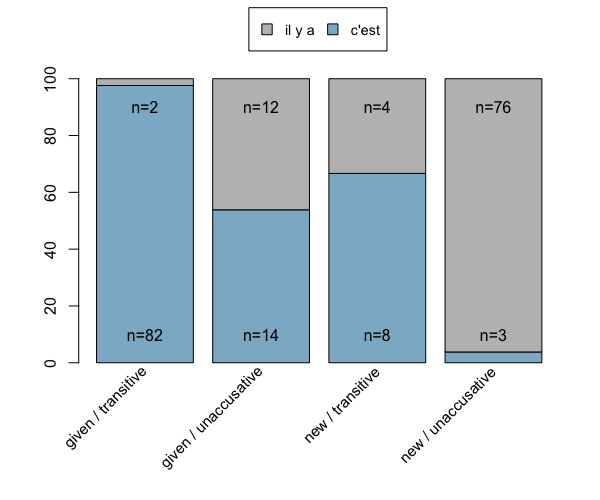
\includegraphics[width=0.7\textwidth]{Images/FR_interaction.png}
    \caption{Interaction of givenness and argument structure}
    \label{fig:5:Plot2}
\end{figure}


Although the model showed no significant interaction effect, observable correlations can still be identified. The given-transitive combination strongly favours the use of a \textit{c'est} cleft, while the new-unaccusative interaction results in a notable majority of \textit{il y a} clefts. In the other two conditions, such tendencies are not as pronounced. When we consider condition 1 (given-transitive) and condition 4 (new-unaccusative), \textit{c'est} and \textit{il y a} clefts appear to behave in opposing ways once again. As demonstrated in earlier sections of this chapter, there exists a ``division of labour” between the two constructions regarding their association with verb types and varying degrees of activation of the subject referent. This section further illustrates that, even when these factors are combined, the preference for a specific cleft format remains robust.


\subsection{Three-factor interaction}
The raw counts presented in Table 16 indicate that some interactions resulted in very few (or no) items, a trend already noted in the Spanish dataset. Nonetheless, it is evident that speakers produced a high number of \textit{c'est} clefts with an exhaustive focus type, a transitive verb, and a given subject.\footnote{Recall that the total of \textit{c'est} clefts analysed here is 107 (not 108), because 1 item had been annotated as ``doubt” regarding its +/- exhaustivity, see section 5.8.1.} Conversely, in the non-exhaustive condition, there is a considerable number of \textit{il y a} clefts associated with unaccusative verbs and new subjects.\\
Given the scarcity of data in the other combinations, it is challenging to determine whether the interaction with focus type significantly impacts the cleft format, assuming all other conditions are equal. For instance, the transitive-given/new association cannot be compared across the exhaustive and not-exhaustive conditions due to the limited items produced.
However, when the verb is unaccusative and the subject is new, there appears to be a tendency to favour the \textit{il y a} cleft, regardless of the type of focus encoded (whether exhaustive or not). Thus, similar to the findings in Spanish, this part of the analysis does not provide clear evidence of whether exhaustivity, in conjunction with the other two predictors, influences cleft choice.



\begin{table}
\begin{tabular}{lllrr}
\lsptoprule
Focus type & Verb type & Information status & \textit{c'est} & \textit{il y a}\\
\midrule
exhaustive & transitive & given & 81 & 1\\
 &  & new & 8 & 1\\
 & unaccusative & given & 14 & 6\\
 &  & new & 3 & 22\\
not-exhaustive & transitive & given & 1 & 1\\
 &  & new & 0 & 3\\
 & unaccusative & given & 0 & 6\\
 &  & new & 0 & 54\\
\midrule
 \textbf{Total} & & & 107 & 94\\
 \lspbottomrule
\end{tabular}
\caption{
% \label{tab:}
Interaction focus type, verb type and information status}
\end{table}

\subsection{Pseudo clefts}
As mentioned previously, due to its scarcity (n=13), pseudo clefts were deemed unsuitable for a statistical analysis with multiple factors or for the formulation of any type of generalization. Therefore, they were excluded from the previous tables. Nevertheless, a qualitative analysis of these structures reveals interesting insights that are discussed in the present section.
Pseudo clefts are discussed in the literature as focus-marking devices associated with specific features, such as syntactic weight of the focused element, containing mostly verbs expressing evaluations, feelings, attitudes, personal opinions or saying verbs \parencite{apotheloz2012pseudo}. Structurally, they exhibit the opposite configuration to \textit{c'est} clefts, in that the background material contained in the relative clause is generally found at the beginning of the utterance, while the clefted element appears at the end. This structural peculiarity has been  claimed to be the reason why these constructions often appear with ``heavy'', long subjects in the clefted element. \\
Cross-linguistically, there is a tendency to avoid placing heavy elements (e.g., clausal subjects) at the beginning of the sentence, and pseudo clefts, due to their configuration, have been reported as an optimal strategy to place the focalized ``heavy” element later in the structure \parencite{prince1978comparison, blanche1990franccais, roubaud2000constructions, calude2009cleft,  apotheloz2012pseudo}. \\
Comparing these observations with the items found in the corpus, it is possible to observe that, indeed, pseudo clefts follow this pattern. The type of subject contained in the clefted element is almost exclusively (in 12 out of 13 cases) a syntactically ``heavy” subject, generally a clausal subject, evidence of what has been previously discussed about these constructions. Only 1 out of 13 cases has been found to contain a subject referent:

\ea \label{ex:5:85}
\ea \textit{Tu peux aller l'interroger}.\\
`You could interrogate her.'
\exi{a.} \textit{Elle aura sûrement des trucs à te dire}.\\
`She will have for sure things to say.'
\ex \textit{Non, moi, ce qui m'intéresse bien, donc, c'est} {[\textit{son mari}]\textsubscript{\textsc{foc}}}\normalsize.\\
`No, me, what interests me the most it's her husband.' \hfill (sgs French, 77/249-251)   
\z \z


The occurrences found in the corpus exhibit a specificational semantics, where the variable \textit{ce qui} or \textit{ce que} contained in the relative clause at the beginning of the structure is filled with the value contained in the clefted element (\textit{c'est X} `it is X'). Given the clausal nature of the focalized subject, it is sometimes not straightforward to determine the type of focus that these constructions express. There seems to be a tendency, though, to encode an exhaustive interpretation of the proposition, and to exclude the other possible alternatives:

 \ea  \label{ex:5:86}
\ea \textit{Il y avait quelque chose qui te laissait prévoir que ce mec, il pourrait avoir des problèmes, ou?} \\
 `Was there something that made you forsee that this man could have problems, or?'
\ex \textit{Ben, moi, ce qui me génait un peu chez lui c'est} {[\textit{le fait qu'il soit rosicrucien}]\textsubscript{\textsc{foc}}} \normalsize \textit{parce que ça lui apportait des fréquentations un peu louches}.\\
‘Well, as for me, what bothered me a little about him is the fact that he was a Rosicrucian, because that meant that he had dangerous acquaintances.' \hfill (sgs French, 78/256-257)   
\z \z 


In (\ref{ex:5:85}), speaker a suggests to speaker b to go interrogate the woman they are talking about. Speaker b, however, answers that s/he is only interested in the husband, excluding his/her interest for the interrogation of the wife. In example (\ref{ex:5:86}), the two speakers are talking about one of the neighbours living in the building. Speaker a is trying to find out if there is something about his personality that could appear suspicious. The interpretation of the pseudo clefts contained in the answer goes more in the direction of `the only thing that bothered me about him was...', suggesting that there were no other aspects of his personality that could result unusual. Thus, in both example (\ref{ex:5:85}) and (\ref{ex:5:86}), it seems that the focalized subject contained in the clefted element of the pseudo clefts excludes all the other possible alternatives.\\
Overall, the pseudo clefts found in the corpus seem to exhibit features that have already been identified by previous research. Their scarcity might be due to the type of data investigated here. More precisely, because pseudo clefts tend to express feelings, personal opinions or emotions, they are not very compatible with a type of dialogue with many fast turns, where speakers are supposed to solve a murder case in an objective way. Rather, this construction type might be more common in traditional sociolinguistic interviews, where speakers utter longer stretches of text, usually relating their personal experiences.\\
Finally, all the 13 items appear with OE-psychological verbs, such as \textit{étonner} `to surprise', \textit{marquer} `to strike', \textit{intéresser} `to interest' and \textit{gêner} `to bother', thus expressing personal feelings and emotions, and almost all the sentences are in the 1st person singular (\textit{moi, je} `I') which grammatically corresponds to the (either direct or indirect) object of the sentence, apart from 2 cases which are impersonal constructions (e.g., \textit{Ce qui est étonnant c'est qu'il avait les clefs} `What is surprising is that he had the keys'). These findings are, once again, in line with previous research.

\section{Comparative analysis}

The findings of this chapter provide several points for both language-internal and comparative discussion. The three factors investigated in relation to the answer type chosen by either Spanish or French speakers appear to influence this choice, albeit to varying degrees. Since information status, verb type, and, at least for French, focus type seem to affect speakers' selection between SV/VS in the Spanish data and between \textit{c'est} and \textit{il y a} clefts in the French data, it is reasonable to assert that the hypothesis formulated in this chapter is partly confirmed.

\subsection{Clefts and exhaustivity}
The results regarding exhaustivity show a strong correlation with specific cleft types only in the French dataset. This finding is not particularly surprising; in the literature on focus, exhaustivity has already been linked to the choice of different cleft formats. In this regard, the results from the French analysis align with what has been claimed by \textcite{de2015status} and \textcite{karssenberg2017oiseaux} regarding the differences between \textit{c'est} and \textit{il y a} clefts when both exhibit the same information-structural partition.\\
Furthermore, the data indicate that exhaustivity is not semantically but rather pragmatically conveyed in these types of clefts. The presence of exclusive focus particles such as \textit{only} and the occurrence of some \textit{c'est} clefts with a not-exhaustive interpretation demonstrate that the implicature of exhaustiveness is cancellable and that such cancellation does not have quantificational effects (i.e., it does not alter the truth-conditional value of the sentence).\\
The correlation between \textit{il y a} clefts and not-exhaustive focus is also not surprising. Authors such as \textcite{de2015status}, \textcite{verwimp2017definite}, and \textcite{karssenberg2017oiseaux} have argued for the ``listing” or ``enumerative” function of these constructions when they exhibit a focus-background partition, where the focused element is generally not the sole value that fills the wh-variable contained in the (either implicit or explicit) Question Under Discussion (QUD), but rather one of several possible options.\\
Moreover, within the exhaustive occurrences of focus, cases of contrast and correction are more frequently found in French \textit{c'est} clefts. Once again, this finding aligns with the results of previous studies on contrast in this language (e.g., \cite{lambrecht1996information}).
While focus type has not yielded statistically significant results for Spanish, the findings for givenness and argument structure are noteworthy: the data demonstrate strong correlations between these factors and specific syntactic structures in both languages.

\subsection{Clefts and argument structure}
As already mentioned, the literature correlating argument structure and clefts in French is almost absent. A closer look, however, reveals that authors such as \textcite{hetzron1975presentative} claim that different cleft formats (at least \textit{c'est} clefts and pseudo) correlate with linear order and with the syntactic function of the argument contained in the clefted element. According to the author's view, \textit{c'est} clefts, because of their configuration, would be ideal strategies to focus the subject because they allow the subject to be placed in an initial-position (which is the most natural position for subjects to appear). Conversely, pseudo clefts serve as effective strategies for focusing the object because the clefted element appears at the end of the utterance. This positioning allows the object to be placed sentence-finally, which is the most common position for objects in sentences. Additionally, according to \textcite{lambrecht1996information}, ``clefts are one specific solution in spoken French to the competition between syntax and pragmatics: different types of clefts allow to preserve a certain linear order of the constituents and guarantee at the same time the pragmatic effect of focus” \parencite[25]{lambrecht1996information}.\\
Building on this assumption, one could argue that this theory applies not only to different syntactic functions but also to various types of subjects. It is well known that subjects are not homogeneous; they make different semantic contributions depending on their level of agentivity and degrees of activation. Consequently, different types of clefts may serve as strategies to encode focus on distinct types of subjects while maintaining the linear order in which these subjects would appear if they were not focalized.\\
However, determining whether this explanation is on the right track is challenging based solely on the current data. The occurrences of pseudo clefts and, to some extent, Spanish \textit{in situ} subjects are too scarce, necessitating a confirmation experiment. Nevertheless, the findings of this chapter and the hypotheses proposed could serve as a foundation for further research on this topic.

\subsection{Focus-marking strategies and ``bad” subjects}
The literature on both Spanish and French focus highlights the fact that the choice of the focus-marking strategies is highly dependent on the the type of subject: light, highly activated subjects, such as pronouns, are better focalized \textit{in situ} through prosodic prominence rather than moved to a postverbal position (e.g., \cite{gabriel2007fokus}). Conversely, long, heavy or brand-new subjects are claimed to be more often found postverbally. Similarly, as mentioned repeatedly, \textit{il y a} clefts are reported as strategies to avoid positioning ``bad” subjects sentence-initially in spoken French \parencite{lambrecht2010constraints, karssenberg20186}. The correlations found in the two sets of data confirm previous claims in this respect.\\
As for argument structure, the strong correlation between the VS order and unaccusative verbs in Spanish is, once again, expected. \textcite{leonetti201724}, for instance, argues that  the distribution of subject inversion reflects a scale of “markedness” that goes from the simplest, core cases of VS with unaccusatives in presentational contexts to the most complex case of inversion with transitive verbs, VSO. Theoretically, the least marked patterns should be the most widespread, while the most marked ones should be the least natural and common.\\
Similarly, the frequent occurrence of subject-verb inversion with unaccusative verbs has been attributed to the absence of agentive properties assigned to their subjects. Authors such as \textcite{contreras1978orden} and \textcite{gutierrez2013structural} claim that different degrees of prominence among thematic roles are reflected in the word order of various languages. Non-prominent roles, such as {\fontfamily{qcr}\selectfont THEMES} or {\fontfamily{qcr}\selectfont PATIENTS}, typically favor inversion, while prominent roles, such as agents, tend to appear sentence-initially.\\
\textcite{gutierrez2013structural} accounts for this phenomenon in terms of ``structural markedness”. He posits that {\fontfamily{qcr}\selectfont THEMES} or {\fontfamily{qcr}\selectfont PATIENTS} in preverbal position are generally considered more marked than {\fontfamily{qcr}\selectfont AGENTS}. Consequently, different languages employ various strategies to mitigate such structural markedness. He considers the VS order in Spanish as one strategy to avoid placing a non-agentive subject in preverbal position.\\
The findings from the Spanish dataset support these claims: the majority of narrowly focused subjects are postverbal subjects of unaccusative verbs. This result may explain why the ``immediacy” hypothesis, formulated in Chapter 4, is only partially confirmed for the Spanish data set. In Chapter 4, the results indicated that when the Question Under Discussion (QUD) immediately preceded the answers, no significant differences were observed in speakers' choices. Unlike French speakers, Spanish speakers opted for both full and elliptical answers. The predominance of full answers in Spanish, which consist of verb + subject, may account for why the repetition of background (BG) material is not perceived as ``heavy” as in French, where the discourse-old proposition is generally encoded by an additional clause.

\subsection{Mapping semantic roles and information-structural functions onto syntax}
Regarding the results of the different interactions, the exploratory analysis — where the three factors interacted — did not yield significant results. The scarcity of data points limits the ability to draw conclusions or make generalizations. Conversely, the confirmatory analysis, which investigated the interaction between verb type and information status, provided intriguing insights.
Among the total \textit{in situ} focused subjects in Spanish, the most frequent combinations involved a given subject with a transitive verb. Similarly, this combination resulted in a majority of \textit{c'est} clefts in French. In contrast, the pairing of unaccusative verbs with new subjects led to a predominance of VS order and \textit{il y a} clefts in Spanish and French, respectively. These correlations are illustrated in Figure 7:\\

\begin{figure}
%     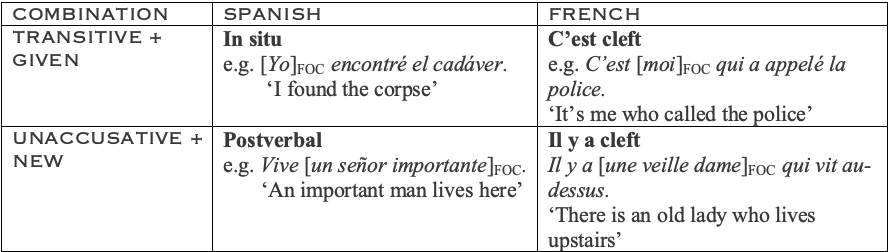
\includegraphics[width=1.0\textwidth]{Images/ES_FR.png}
    \small
    \begin{tabularx}{\textwidth}{p{2.5cm}QQ}
      \lsptoprule
      Combination & Spanish & French \\
      \midrule
      TRANSITIVE + GIVEN & \textbf{in situ}\newline
                          e.g. \textit{[Yo]\textsubscript{\textsc{foc}} encontré el cadáver}\newline
                          `I found the corpse.' &
                              \textbf{C'est cleft}\newline
                              e.g. \textit{C'est [moi] qui a appelé la police}\newline
                              `It's me who called the police.'\\
\tablevspace
      UNACCUSATIVE + NEW & \textbf{Postverbal} \newline
                           e.g. \textit{Vive [un señor importante]\textsubscript{\textsc{foc}}}\newline
                          `An important man lives here'&
                              \textbf{Il y a cleft} \newline
                              \textit{Il y a [une vieille dame]\textsubscript{\textsc{foc}} qui vit au-dessus.}\newline
                              `There is an old lady who lives upstairs.'\\
      \lspbottomrule
    \end{tabularx}
\todo[inline]{Check `C'est moi qui \textbf{ai} appelé la police'.}
\todo[inline]{Check where the `here in the translation of `An important man' comes from.}
    \caption{Comparative overview of Spanish and French correlations}
    \label{fig:5:Plot3}
\end{figure} 


According to \textcite{lambrecht2010constraints}, grammars reflect universal cognitive constraints on the mapping between the informational structuring of utterances, the semantic structuring of propositions, and the formal structuring of sentences. These constraints restrict the possible
alignments among the following pragmatic, semantic, and syntactic parameters:
\begin{itemize}
    \item pragmatic relations (topic and focus)
    \item pragmatic statuses of discourse referents (hearer-new vs. hearer-old, discourse-new vs. discourse-old)
    \item semantic roles (agent and patient)
    \item grammatical relations (subject and object)
    \item syntactic positions (e.g., preverbal vs. postverbal position in SVO languages)
\item morphosyntactic and prosodic forms
\end{itemize}


In other words, there are clearly visible tendencies across languages where certain features reflect syntactic structures. Specifically, given arguments tend to precede new ones, {\fontfamily{qcr}\selectfont AGENTS} appear before {\fontfamily{qcr}\selectfont PATIENTS}, subjects come before objects, and topics are positioned before foci. However, Lambrecht does not explain how these elements interact and how this interaction is resolved in syntax.
In this chapter, I tested the interaction between several of these features: subjects that are also foci, varying levels of agentivity, and degrees of givenness.\\
The results indicate that being a given {\fontfamily{qcr}\selectfont AGENT} promotes its placement in sentence-initial position, while being unagentive (due to the presence of an unaccusative verb) and brand-new favors postverbal placement. The typological differences between Spanish and French lead to variations in this placement; in Spanish, it is resolved through word order (SV/VS), whereas in French, it is managed through two different construction strategies: \textit{c'est} and \textit{il y a} clefts.
In Spanish, this mapping is more straightforward. In French, however, it requires additional explanation. As illustrated in Figure 7, a \textit{c'est} cleft, due to its syntactic configuration, allows the subject to be positioned early in the sentence, while the object is placed at the end. Conversely, as noted by \textcite{lambrecht2010constraints}, an \textit{il y a} cleft serves as an optimal strategy to delay the appearance of the subject. This strategy aligns with the spoken French constraint of avoiding placing brand-new subjects at the beginning of a sentence, thus positioning them later in the structure.\\
One might argue that, unlike the Spanish SV structure, the subject in a \textit{c'est} cleft does not appear at the very beginning of the sentence. Instead, it is introduced by a non-referential pronoun and a copula. This could be attributed to the fact that clefts have become grammaticalized structures. Both the copula and the relative pronoun can be considered semantically light and function as ``discontinuous grammatical morphemes that serve the pragmatic function of focus marking” \parencite[197]{wehr2011phrase} or as morphological focus markers in the form of a ``circumfix” \parencite[126]{haase2000franzosische}.

\subsection{The case of pseudo clefts}
Finally, in the case of pseudo clefts, their unique structural configuration allows the focused subject to be positioned at the end of the sentence, preceded by the relative clause that typically constitutes the background (BG) material. In the corpus, pseudo clefts are rare but are always accompanied by OE-psych verbs. Observing these types of verbs in other Romance languages, such as Spanish or Italian, reveals a special syntactic word order where the (direct or indirect) object precedes the verb and the subject, resulting in an OVS order (e.g., \textit{A Ester no le gustan estas fiestas} `Esther doesn’t like these types of parties').\\
Theories of thematic prominence have attributed this special configuration to the fact that the subject selected by these types of verbs is not the prototypical {\fontfamily{qcr}\selectfont AGENT} but rather the {\fontfamily{qcr}\selectfont STIMULUS} of the sentence, that provokes feelings and emotions to the object, who has the thematic role of {\fontfamily{qcr}\selectfont EXPERIENCER}. In these theories, the {\fontfamily{qcr}\selectfont EXPERIENCER} is considered to have more agentive properties than the {\fontfamily{qcr}\selectfont STIMULUS} \parencite{gutierrez2013structural},\footnote{This is also due to the fact that the {\fontfamily{qcr}\selectfont EXPERIENCER} is, by definition, an animate entity, while the {\fontfamily{qcr}\selectfont STIMULUS} can either be animate or inanimate.} and is therefore placed in a position higher in the structure because of the mapping constraints identified by \textcite{lambrecht2010constraints}. Observing again the syntactic configuration of pseudo clefts, it is possible to see that, when accompanied by OE-psych verbs, a pseudo cleft allows the positioning of an argument that is the object-experiencer in a higher position than the subject stimulus (e.g., \textit{Ce qui \textbf{m'}intéresse bien, donc, c'est \textbf{{son mari}}} `What interests me more is her husband').\\
Thus, the difference in syntactic positions or cleft types in Spanish and French respectively can be captured in terms of features, such as agentivity level and activation state of the argument(s) in the sentence. In line with \textcite{lambrecht2010constraints}, syntactic variation seems to reflect universal cognitive constraints. The occurrence of different variants in the same pragmatic context could be due to the different semantic contributions of the subject, and the findings reported in this chapter provide evidence of the fact that such constraints are also visible in interaction with focus.

\subsection{Additional cross-linguistic evidence}
To highlight even more the importance of argument structure in focus realization, it is possible to look cross-linguistically at languages where change is ``in progress”. In Brazilian Portuguese (BP), for instance, a language well known for being in a transitional phase, two main focus-marking strategies are reported for the subject: clefts sentences \textit{à la} French and postverbal subjects \textit{à la} Spanish. Interestingly, their alternation is claimed to be linked to the verb type contained in the sentence \parencite{kato2006focus}: speakers tend to choose it-clefts for transitive verbs, while postposed subjects are maintained with monoargumental verbs, as in (\ref{ex:5:87}) and (\ref{ex:5:88}):\\

\ea \label{ex:5:87} Brazilian Portuguese
\ea \textit{O João telefonou?}\\
 ‘Did John call?'
\ex  \textit{Não. Telefonou} {[\textit{o PEDRO}]\textsubscript{\textsc{foc}}}\normalsize.\\
‘No, Peter called.' \hfill \parencite[9]{kato2006focus}    
\z \z

\ea \label{ex:5:88}
\textit{É} {[\textit{o Pedro}]\textsubscript{\textsc{foc}}} \normalsize \textit{que ama a Maria}.\\
`It is Peter who loves Maria.’ \hfill \parencite[10]{kato2006focus}   
\z


Thus, BP can be considered, in this respect, a hybrid variety between two different languages (e.g., French and Spanish) with a different typology with respect to focus realization, where the alternation between different focus-marking strategies is strictly dependent on argument structure of the verb.

\section{Summary}
In this chapter, I have tested and discussed factors previously claimed to impact focus realization in both Spanish and French. These factors have often been investigated separately and not in their interactions, making this study a novel contribution to the field. It demonstrates that the interplay between certain aspects of information status and argument structure significantly affects the choice of focus-marking strategies in both languages. Notably, the role of argument structure has not been analysed in correlation with cleft sentences before.
I formulated the hypothesis that the three factors investigated — focus type, information status of the subject referent, and argument structure — are reflected differently in Spanish and French due to their typological differences in encoding focus. In Spanish, the influence of these factors is evident in word order alternation, particularly in the position of the subject. In contrast, French, with its relatively rigid word order, exhibits the impact of the same factors through the choice of cleft format.\\
Although focus type was not found to have a significant impact on the Spanish data, the hypothesis is still partly confirmed. The roles of givenness and argument structure, however, are clearly visible in the data, with strong correlations: given subjects of transitive verbs are predominantly encoded as preverbal subjects in Spanish and as \textit{c'est} clefts in French, while new subjects of unaccusative verbs are most commonly represented by postverbal subjects and \textit{il y a} clefts.
To find common ground between the two languages, I have linked these tendencies to theories suggesting that specific features map onto specific syntactic positions. Such an analysis, however, has several limitations. Certain interactions between factors could not be observed due to the low number of data points. It would be beneficial to conduct experimental studies, such as forced-choice tasks or acceptability judgments, with selected stimuli in a more controlled experimental setting. I leave this for further research.
